%%%%%%%%%%%%%%%%%%%%%%%%%%%%%%%%%%%%%%%%%%%%%%%%%%%%%%%%%%%%%
% ECE 445 SENIOR DESIGN TEMPLATE
%%%%%%%%%%%%%%%%%%%%%%%%%%%%%%%%%%%%%%%%%%%%%%%%%%%%%%%%%%%%%
\documentclass[openbib,letterpaper,10pt]{article}

%%%%%%%%%%%%%%%%%%%%%%%%%%%%%%%%%%%%%%%%%%%%%%%%%%%%%%%%%%%%%
% The preamble starts here.
% You can add other packages that you want to use by using
% \usepackage command in the preamble.
% However, DO NOT change the settings that are already placed
% below unless you really know what you are doing.
%%%%%%%%%%%%%%%%%%%%%%%%%%%%%%%%%%%%%%%%%%%%%%%%%%%%%%%%%%%%%

% some commonly used packages
\usepackage{graphicx}
\usepackage{color,soul}
\usepackage{amsmath}
\usepackage{amsthm}
\usepackage{amsfonts}
\usepackage{setspace}
\usepackage{longtable}
\usepackage{url}
\usepackage{float}
\usepackage{caption}
\usepackage[colorlinks=true,linkcolor=black,citecolor=black]{hyperref}
\usepackage[top=1in, bottom=1in, left=1in, right=1in]{geometry}% set the page margins to 1 inch

% use the fancyhdr package to maintain the format of the page numbers,
% which is useful when the text color is changed
\usepackage{fancyhdr}
\fancyhf{}
\renewcommand{\headrulewidth}{1pt}
\renewcommand{\footrulewidth}{0pt}
\fancyfoot[C]{\textcolor{black}{\thepage}}
\fancyhead[L]{
\includegraphics[width=2cm]{University-of-Illinois-logo.jpg}}
\fancyhead[R]{\small{Infantry I.F.F. Mock Design Review - Meyers \& Prince}}

% paralist provides extended list environments
\usepackage{paralist}
\setlength{\plitemsep}{0pt}

% define the color for section and subsection titles
\usepackage{xcolor}
\definecolor{titlecolor}{RGB}{31,73,125}
\definecolor{subtitlecolor}{RGB}{79,129,189}

% tikz/pgf environment for making graphs
\usepackage{tikz}
\usepackage{tikz-timing}[2009/12/09]
\usetikzlibrary{shapes,arrows}
\usetikztiminglibrary[new={char=Q,reset char=R}]{counters}

% change the style of the abstract environment
\usepackage{abstract}
\setlength{\absparsep}{6pt}
\setlength{\absleftindent}{0pt}
\setlength{\absrightindent}{0pt}
\setlength{\abstitleskip}{-18pt}
\renewcommand{\absnamepos}{flushleft}
\renewcommand{\abstractnamefont}{\normalfont\Large\singlespacing\bfseries}
\renewcommand{\abstractname}{\textcolor{titlecolor}{Abstract}}

% change the style of the section and subsection titles
\usepackage{titlesec}
\titleformat{\section}{\color{titlecolor}\Large\bf}{\color{titlecolor}\thesection}{0.8em}{}
\titleformat{\subsection}{\color{subtitlecolor}\large\bf}{\color{subtitlecolor}\thesubsection}{1em}{}
\titleformat{\subsubsection}{\color{subtitlecolor}\normalsize\bf}{\color{subtitlecolor}\thesubsubsection}{1.2em}{}
\titlespacing{\section}{0pt}{0em}{0em}
\titlespacing{\subsection}{0pt}{0em}{0em}
\titlespacing{\subsubsection}{0pt}{0em}{0em}

% change the style of the table of contents
\usepackage{titletoc}
\titlecontents{section}[1.5em]{}{\contentslabel{1.5em}}{\hspace*{-1.5em}}{\titlerule*[0.5pc]{.}\contentspage}
\titlecontents{subsection}[3em]{}{\contentslabel{2.1em}}{\hspace*{-2.1em}}{\titlerule*[0.5pc]{.}\contentspage}
\titlecontents{subsubsection}[5.1em]{}{\contentslabel{2.7em}}{\hspace*{-2.7em}}{\titlerule*[0.5pc]{.}\contentspage}

% command for centering texts in a fixed width table cell
\newcommand{\centpcol}{\leftskip\fill \rightskip\fill}

% command for setting the style of the appendix titles
\newcommand{\setappenstyle}{
	\titleformat{\section}{\color{titlecolor}\Large\bf}{\color{titlecolor}Appendix \Alph{section}}{0.8em}{}
	\titlecontents{section}[0em]{}{Appendix \thecontentslabel \hspace{1em}}{}{\titlerule*[0.5pc]{.}\contentspage}
}

% define the style of the title of the paper
\newcommand{\thetitle}[1]{\title{\begin{huge}{\bf #1}\end{huge} \color{subtitlecolor}\rule[25pt]{\textwidth}{1pt}}}

% define the style of the author
\newcommand{\theauthor}[3]{
	\author{\vspace{.4in}\\
	\textcolor{black}{By}\\
	#1
	\vspace{1in}\\
	\textcolor{black}{ECE 445 Mock Design Review -} #2\\
	\textcolor{black}{TA:} #3
	\vspace{1in}}
}

% define the style of figure's caption
\newcommand{\figcap}[1]{
	\captionsetup{format=plain,font={small,color=subtitlecolor,singlespacing},margin={0pt,0pt}}
	\caption{\textcolor{subtitlecolor}{#1}}
	\vspace{-5pt}
}

% define the style of table's caption
\newcommand{\tablecap}[1]{
	\captionsetup{format=plain,font={bf,normalsize,singlespacing,color=black},margin={0pt,0pt}}
	\caption{\textcolor{black}{#1}}
	\vspace{-5pt}
}

% define the style of the abstract's page number
\newcommand{\abstractsetting}{
	\pagenumbering{roman}
	\thispagestyle{fancy}
}

\newcommand{\buildtoc}{
	\clearpage
	\singlespacing
	\tableofcontents
	\onehalfspacing
}

% set indentations and the space between paragraghs
\setlength{\parindent}{0pt}
\setlength{\parskip}{8pt}

%%%%%%%%%%%%%%%%%%%%%%%%%%%%%%%%%%%%%%%%%%%%%%%%%%%%%%%%%%%%%
% PREAMBLE ENDS HERE, DOCUMENT STARTS BELOW
%%%%%%%%%%%%%%%%%%%%%%%%%%%%%%%%%%%%%%%%%%%%%%%%%%%%%%%%%%%%%

\begin{document}

% don't change these
\pagestyle{empty}
\doublespacing

% put the title of your project here. DO NOT include the brackets.
\thetitle{{I.F.F. (Identification Friend or Foe) System}}

% put your names here. seperate by \\. DO NOT include the brackets.
\theauthor{
	{Eric Meyers (emeyer7)}\\
	{Noah Prince (nprince2)}\\
}
{ % put the semester info here. DO NOT include the brackets.
	{Spring 2016}
}
{ % put your TA's name here. DO NOT include the brackets.
	{Braedon Salz}
}

% put the date and project number here. DO NOT include the brackets.
\date{
{February 18th, 2016}\\
Project No. 11
\clearpage
}

% don't change these
\maketitle
\pagestyle{fancy}
\begin{spacing}{1.15}


% build the table of contents. 
\color{black}
\buildtoc
\pagenumbering{gobble}
\section*{Acronyms \& Pre-Requisite Information}
\begin{itemize}
	\item MCU - Microcontroller Unit
	\item R.F. - Radio Frequency
	\item T.I. - Texas Instruments
	\item 
\end{itemize}
\clearpage
\setcounter{page}{1}
\pagenumbering{arabic}

%SECTION 1 - Introduction - Eric
\section{Introduction}
This document is a "Mock Design Review" in preparation for the Design Review occuring during the week of February 29th, 2016. This will better prepare the team for documentation of the design and construction of the Infantry I.F.F. System.

%SECTION 2 - Design - Eric
\section{Block Diagram}
\begin{figure} [H]
	\centering
	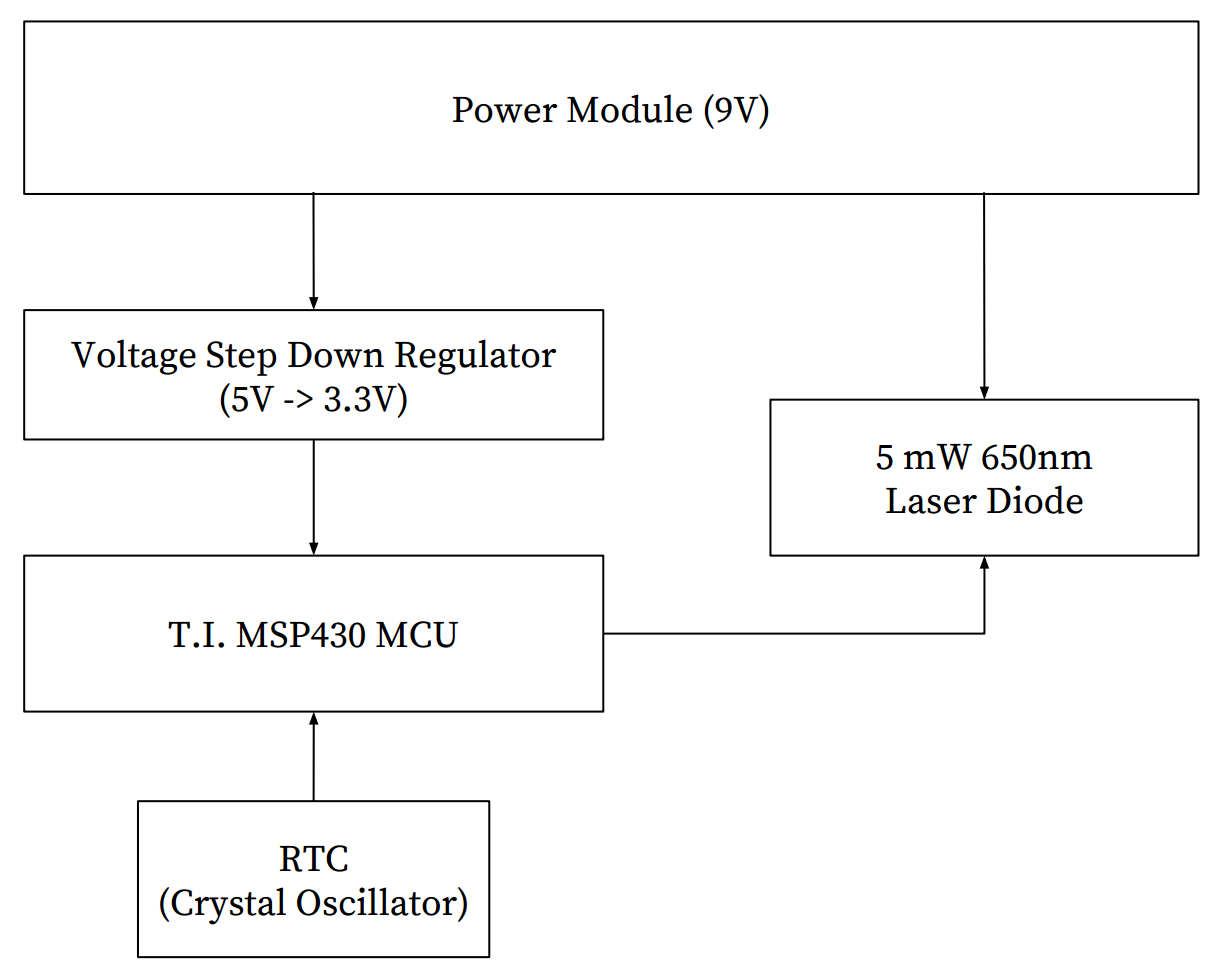
\includegraphics[scale=0.50]{Block_Diagram.png}
	\caption{Block Diagram of Laser Transmitter\label{fig:circuit-schematic}}
\end{figure}

%SECTION 5 - Block Description - Eric
\section{Block Description}
The subsystem of the Laser Transmitter will be broken down into 5 primary modules:
\begin{enumerate}
	\item Power Module
	\item Voltage Step Down Regulator
	\item Microcontroller 
	\item Real Time Clock
	\item Laser Diode
\end{enumerate}

\subsection*{Power Module}
The Power Module will consist of a standard 9V battery. The type of battery is at the discretion of the operator due to the availability on the market. However, at battery with least 250 mAh of use time must be selected to supply the circuit with 9V over a period of 8 hours. The team will chose to use a 9V 300 mAh NiMH Rechargable Battery for testing purposes.

The team decided to use a 9 V battery instead of four double-A batteries due to the need of maintaining a constant 3.3V over time as well as...

ADD MORE

\subsection*{Voltage Step Down Regulator}
The voltage step-down regulator will take the 9V supply input and step it down to 3.3V to supply the MSP430 MCU

ADD MORE

\subsection*{Microcontroller}
This design choice was by far the most difficult. 

ADD MORE

\subsection*{Real Time Clock}
The Real Time Clock is not entirely neccessary for the operation of the Laser Transmitter Subsystem, however it will be neccessary for the operation of the R.F. Receiver and thus must be included in the MCU circuit.

ADD MORE

\subsection*{Laser Diode}
The laser diode...

ADD MORE


\clearpage

%SECTION 3 - Circuit Schematic - Eric
\section{Circuit Schematic}
\begin{figure} [H]
	\centering
	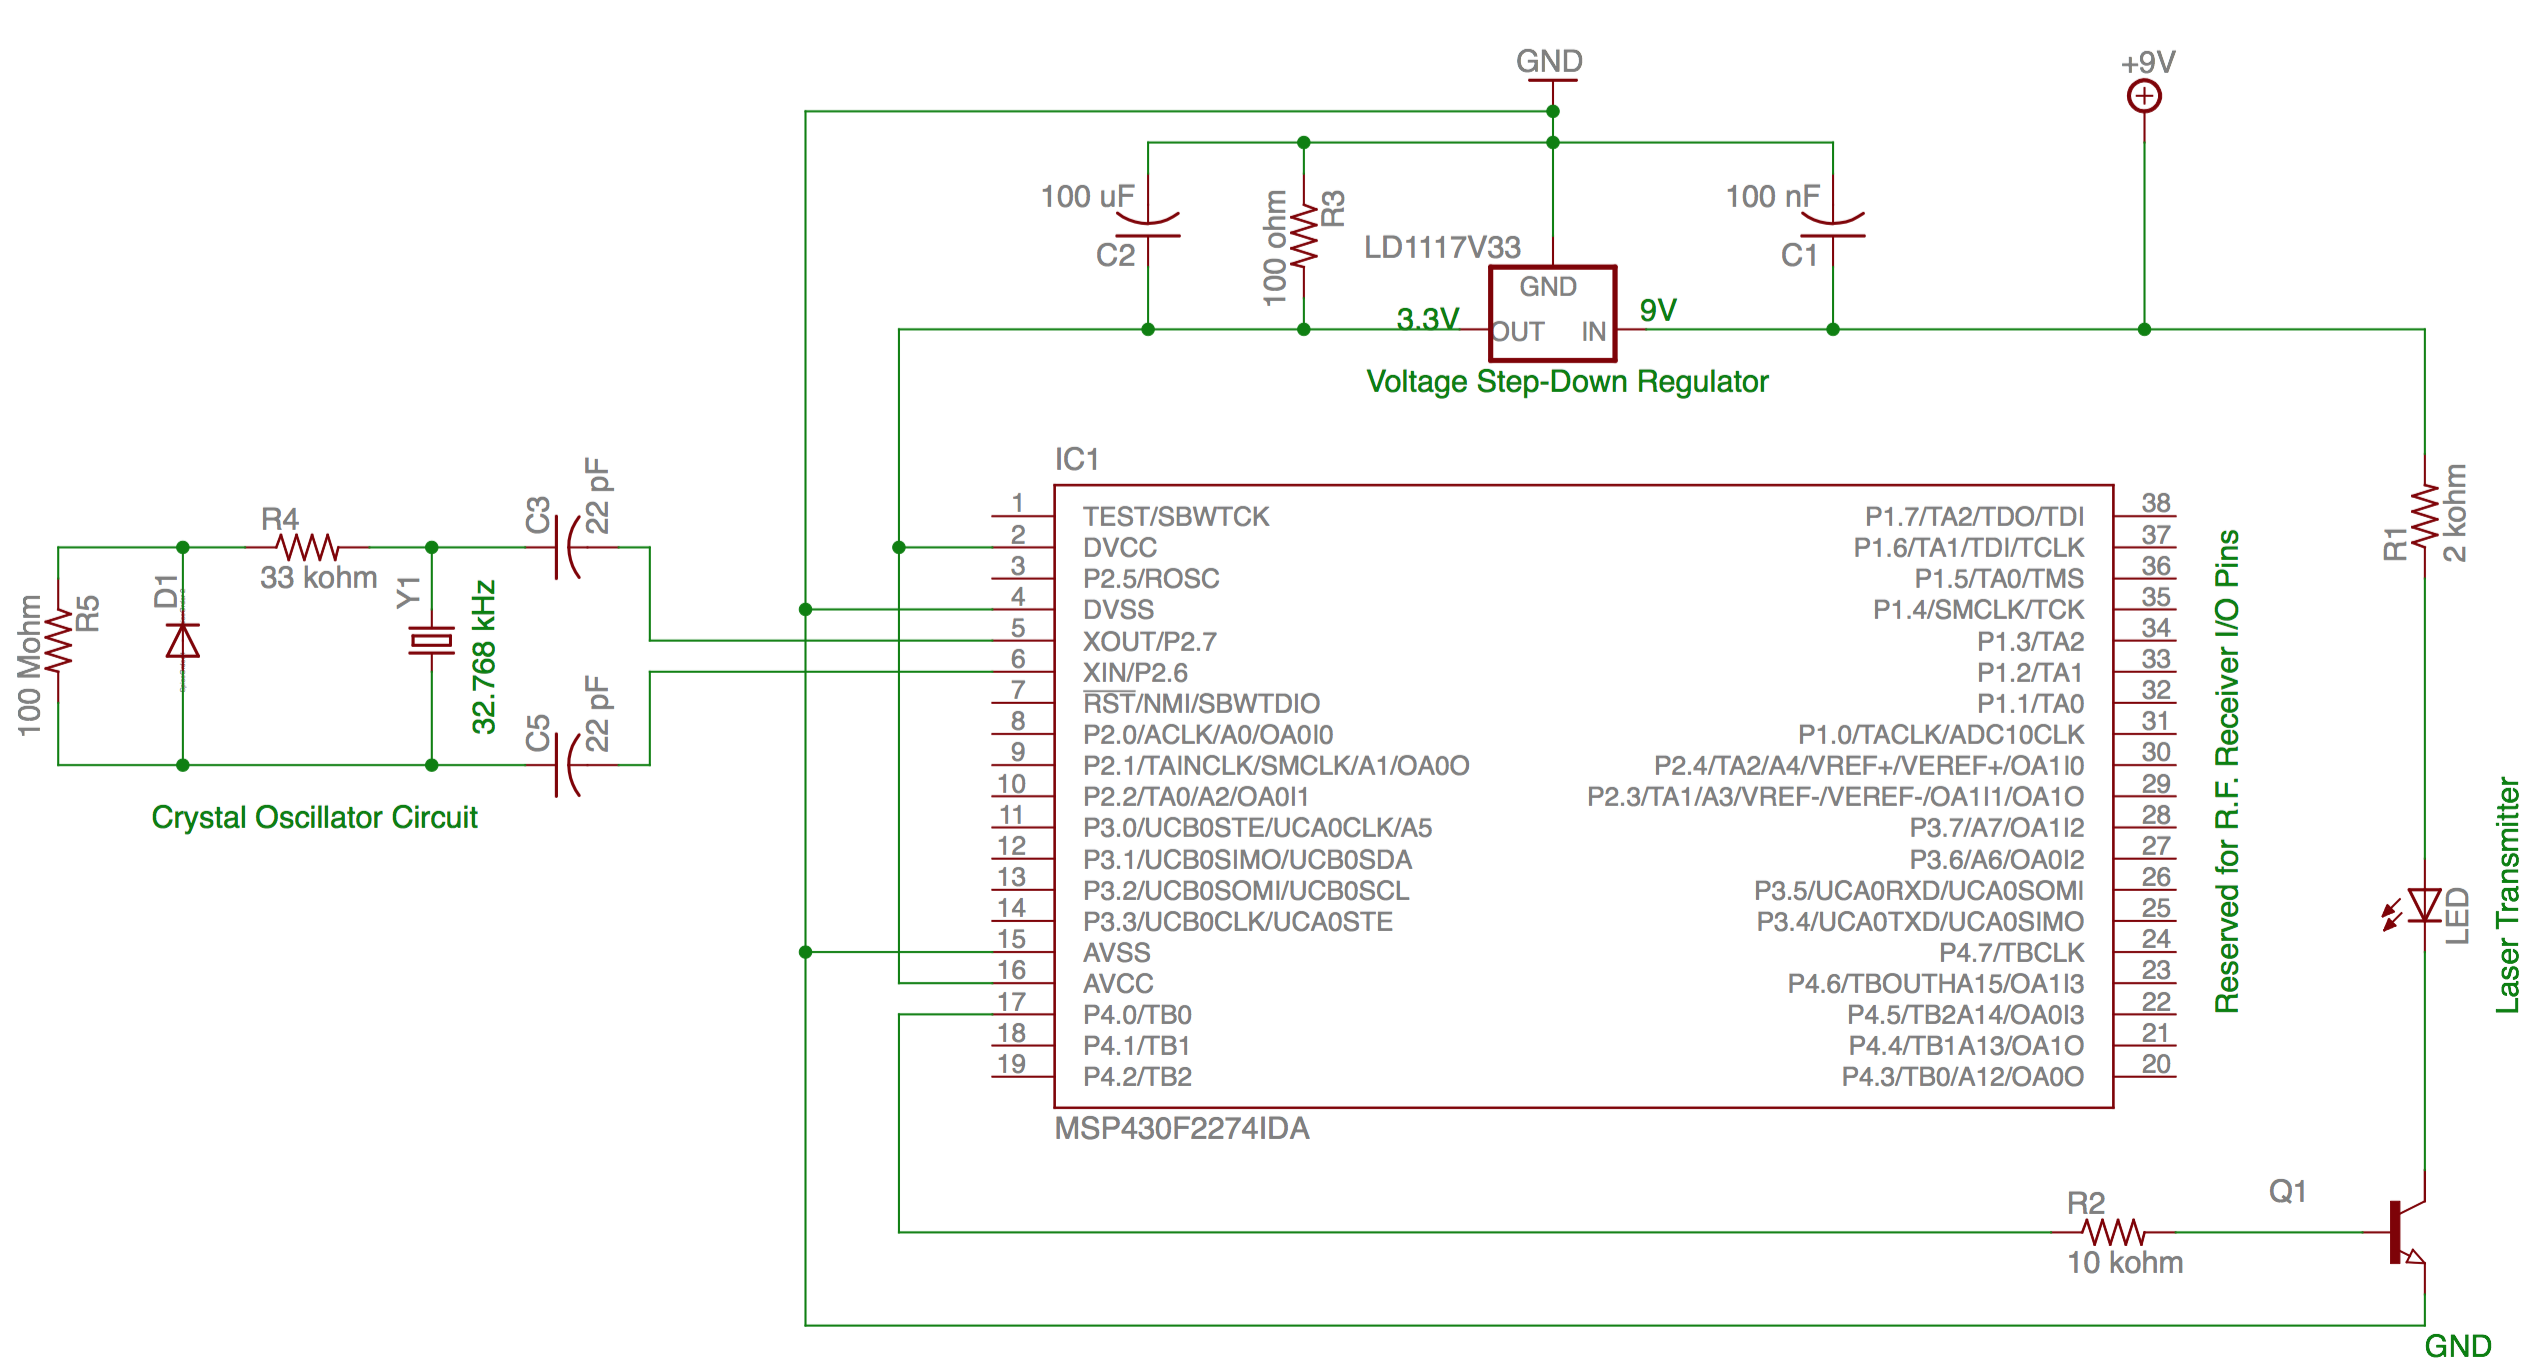
\includegraphics[scale=0.38]{Circuit_Schematic.png}
	\caption{Circuit Schematic of Laser Transmitter\label{fig:circuit-schematic}}
\end{figure}

%SECTION 4 - Plot/Experiment - Noah
\section{Plot}
NOAH SECTION

%SECTION 5 - Requirements and Verification - Both 
\section{Requirements and Verification}
FILL OUT TOGETHER

%SECTION 6 - Safety - Noah
\section{Safety \& Ethical Considerations}
NOAH SECTION

\clearpage
\bibliographystyle{IEEE_ECE}
% include the BibTex file here to build reference
\bibliography{Citations}\addcontentsline{toc}{section}{Reference}

\clearpage
\end{spacing}
\end{document}

